% Use a one-sided article template
\documentclass[oneside]{article}
% Decrease the margins a little
\usepackage{fullpage}

% Set up for including graphics
% We'll use png or pdf graphics
\usepackage[pdftex]{graphicx}
\DeclareGraphicsExtensions{.png,.pdf}

% Hyperref adds hyperlinks to the document automatically
% It's not much use yet, but it will be
\usepackage{hyperref}

% For including code into the document
\usepackage{verbatim}

% Tweak the default fonts a little
\renewcommand\rmdefault{bch}
\usepackage[small]{caption}
\usepackage[small]{titlesec}
\linespread{1.07} 

\title{Stat640 - Progress Report 1}
\author{Matt Delhey \& Frank Portman}
\date{\today}

\raggedbottom
\pagestyle {empty}

\begin{document}

\begin{center}
\textbf{Stat640 - Progress Report 1 - Charlemagne and the Carolingian Empire (Delhey/Portman)}
\end{center}

\begin{figure}[htbp]
  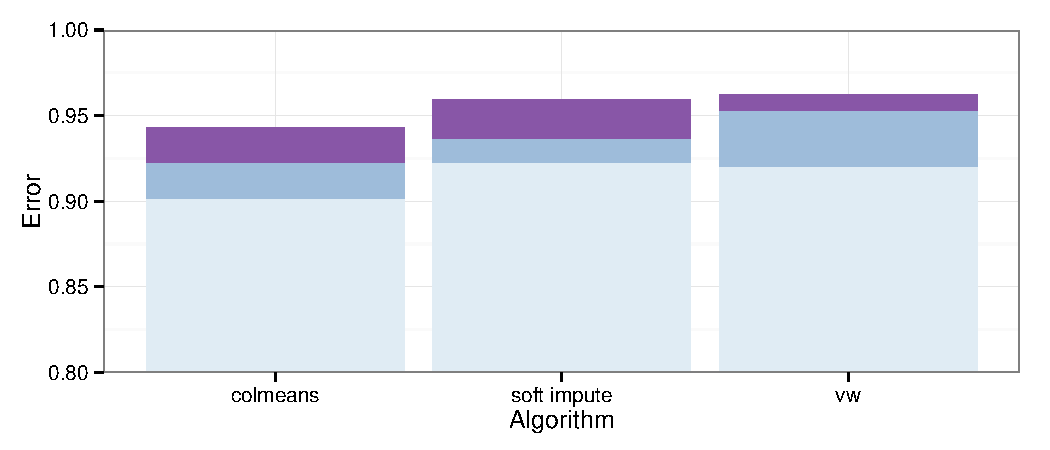
\includegraphics[width = 1.0\linewidth]{vis}
\end{figure}

\begin{description}
\item[What learning algorithms have you tried? Reflect upon the performance.] So far in the competition we have primarily tried implimenting three methods:
  \begin{itemize}
  \item \textbf{colmeans}
  \item \textbf{vw}
  \item \textbf{soft impute}
  \end{itemize}

\item[Actual performance of algorithms. Which ones worked well? Which performed poorly? Why?]

\item[Project organization.] In order to deal with the inevitable technical problems of colobration, our team has setup a github repository to share code and results. We've also both setup DAVinCI accounts and succesfully ran jobs on the cluster. Looking forward, we are in the process of creating a shared folder on DAVinCI and plan on utalizing the cluster for future computations.

\item[Have you innovated? If so, how?]

\item[What are the future direction in which you would like to go?]
\end{description}

\end{document}